\section{Humanity in the Anthropocene}

\subsection{The Secret History of Silicon Valley}

\begin{itemize}
    \item Terman/Stanford/Government responsible for entropreneurial culture
        of Silicon Valley.
    \item Military primed the pump as a customer for key Valley technologies
        \begin{itemize}
            \item Semiconductors, computers, Internet
            \item But very little technical cross pollination
        \end{itemize}
    \item Venture Capital turned the valley to volume corporate and consumer
        applications
    \item Berkeley continued its focus on Big Science and National Labs
\end{itemize}

\subsubsection{Story 1: WW\uproman{2} The First Electronic War}

\paragraph{The German Air Defense System: The Kammhuber Line}

\begin{itemize}
    \item Integrated Electronic air defense network
    \item Protection from British/US bomber raids (Warn and detect, target
        and aim, destroy)
\end{itemize}

\paragraph{British/American Air War in Western Europe}

28'000 active Combat Planes, 40'000 Allied planes lost or damaged beyond
repair: (46'000 planes lost by the USSR in the East), 160'000 Americans and
British killed, wounded or captured.

\paragraph{Mammoth Early Warning Radar}

200 mile range, 100' wide, 33' high, 1st phased-array radar, Operational 1942,
20 built

\paragraph{Wasserman Early Warning Radar}

150 mile range, Backbone of the German early warning network, steerable tower
190', operational 1942, 150 built

\paragraph{German Night-Fighters}

Airborne Intercept Radar, Directed to vicinity by ground radar, Allowed the
german fighters to find the bombers at night.

\vspace{1\baselineskip}

By August 1941 only 10\% of Britisch bombers got within 10 miles of their
target.

\subsubsection{Story 2: The Electronic Shield-Electric Warfare}

\paragraph{Harvard Radio Research Lab (RRL) Signals Intelligence and Electronic
Warfare}

\begin{itemize}
    \item Reduce losses to fighters and flak
    \item Find/understand German Air Defense (Electronic and Signals Intelligence)
    \item Jam/confuse German Air Defense
        \begin{itemize}
            \item Radar Order of Battle
            \item Chaff (strips of metal foil released in the air to obstruct
                radar detection)
            \item Jammers
        \end{itemize}
    \item Top Secret 800 person lab
\end{itemize}

\paragraph{Who ran this secret lab and became the Father of Electronic Warfare?}

\begin{itemize}
    \item Harward Radio Research Lab
    \item Director: Fredrick Terman - Stanford
    \item Stanford Professor of engineering 1926
        \begin{itemize}
            \item encouraged his students, William Hewlett and David Packard to
                start a company
        \end{itemize}
    \item Dean of Engineering 1946
    \item Provost 1955
\end{itemize}


\subsubsection{Story 3: Stanford and the Cold War}

\paragraph{Terman's Postwar Strategy}

\begin{itemize}
    \item Focus on microwaves and electronics (did not want to get left out
        in Government spending)
    \item Recriuts 11 former members of RRL as faculty
    \item Set up the Electronics Research Laboratory (ERL)
        \begin{itemize}
            \item "Basic" and Unclassified Research
        \end{itemize}
    \item First Office of Naval Research (ONR) contract 1946
    \item By 1950 Stanford was the MIT of the West
\end{itemize}
RRL = radio research laboratory at Harvard

\paragraph{Microwave Valley - Stanford Spinouts}

There were many spinoffs from Stanford that focused on Mictowaves.
Especially microwave tube startups and other microwave components.

\paragraph{The Cold War and Stanford}

\begin{itemize}
    \item The Cold War battlefield moves 500 miles east
    \item Countermeasures, ELINT become critical
    \item Stanford becomes a center of excellence for the CIA, NSA, Navy, Air
        Force
    \item 400-person weapons lab in engineering department
\end{itemize}
ELINT = electronic intelligence

\paragraph{The Cold War is an Electronic War}

\begin{itemize}
    \item Russian air defense modeled after Germans
        \begin{itemize}
            \item add surface to air missiles, fighter radar, IFF
            \item Understand and defeat (ELINT)
        \end{itemize}
    \item Soviet strategic missile and bomber threat
        \begin{itemize}
            \item Monitor telemetry (SIGINT) to understand performance
            \item Photo reconnaissance to find silo's and bombers
        \end{itemize}
    \item Soviet Naval threat
        \begin{itemize}
            \item Monitor and track soviet submarines
        \end{itemize}
    \item Soviet Nuclear threat
        \begin{itemize}
            \item Identify and understand production facilities
        \end{itemize}
\end{itemize}
Identification, friend or foe (IFF) is a radar-based idendification system
designed for command and control. It enables military and civilian aif traffic
control interrogation systems to identify aircraft, vehicles or forces as
friendly and to determine their bearing and range from the interrogator.

SIGINT = signal intelligence


\paragraph{Stanford joins the "Black" World}

\begin{itemize}
    \item Electronics Research Laboratory ("Basic" and Unclassified Research)
    \item Applied Electronic Laboratory (AEL) ("Applied" and Classified programs)
    \item Merge and become the Systems Engineering Lab (SEL) in 1955 (Same year
        Terman becomes Provost)
    \item Immediate, practical application of real world intelligence problems
        for CIA, NSA, NRO, Air Force
    \item Combined ERL components with advanced theory into complete SIGINT
        and Jamming systems
        \begin{itemize}
            \item Usually prototypes turned over to contractors
            \item At times, built one-off systems
            \item Degital filtering, OTH (over the horizon), etc
        \end{itemize}
    \item Use PhD students and staff (classified thesis!)
    \item Ultimately 800 person lab
\end{itemize}

\paragraph{Terman Changes the Startup/University Rules}

\begin{itemize}
    \item Graduate students encouraged to start companies
    \item Professors encouraged to consult for these companies
    \item Terman and other professors take board seats
    \item Technology transfer/IP licensing easy
    \item Getting out in the real world was good for your academic career
    \item Failure was accepted as part of the culture
\end{itemize}

\paragraph{Stanford/Military/Industry Ecosystem}

\begin{itemize}
    \item Stanford did basic research in electronics
    \item Stanford and SRI do applied research
    \item Microwave and systems companies in Silicon Valley produce equipment
        for the military
\end{itemize}

\paragraph{Terman's Strategy}

\begin{enumerate}
    \item Sit on every possible Military Advisory board
        \begin{itemize}
            \item Build Network and relationships
        \end{itemize}
    \item Reach out to military customers to understand their needs. Then craft
        a prototype in Stanford's labs
        \begin{itemize}
            \item generate revenue for the university and strenghten its
                military relationship
        \end{itemize}
    \item If the customer liked the prototype, encourage a student to found
        a company and manufacture at scale
        \begin{itemize}
            \item inspired entrepreneurship (and hard work) in the students in
                the university's labs
        \end{itemize}
    \item Put a Stanford faculty (or Terman) on the board or as a consultant
        with the new company
        \begin{itemize}
            \item This trained Stanford faculty in business and turned them into
                better teachers and researchers
        \end{itemize}
    \item Provide office space in the Stanford Industrial Park
        \begin{itemize}
            \item This ensured that the startup stayed close and helped the
                entrepreneurial ecosystem reach a higher density
        \end{itemize}
\end{enumerate}

\paragraph{Consequences for Stanford}

\begin{enumerate}
    \item Stanford became the preferred contractor for ELINT and Electronic
        Warefare (EW) prototypes
        \begin{itemize}
            \item Frederick Terman was a ELINT and EW gatekeeper
        \end{itemize}
    \item Stanford attracted talented students, military customers, and
        later, private investor ecosystem
    \item Academic research in ELINT and EW was driven by customers' needs
        rather than being pushed by lab or the agendas of national research
        agencies
        \begin{itemize}
            \item Terman as the first advocate for Customer Development
        \end{itemize}
\end{enumerate}

\paragraph{Microwave Valley - Systems}

\

\begin{figure}[H]
    \centering
    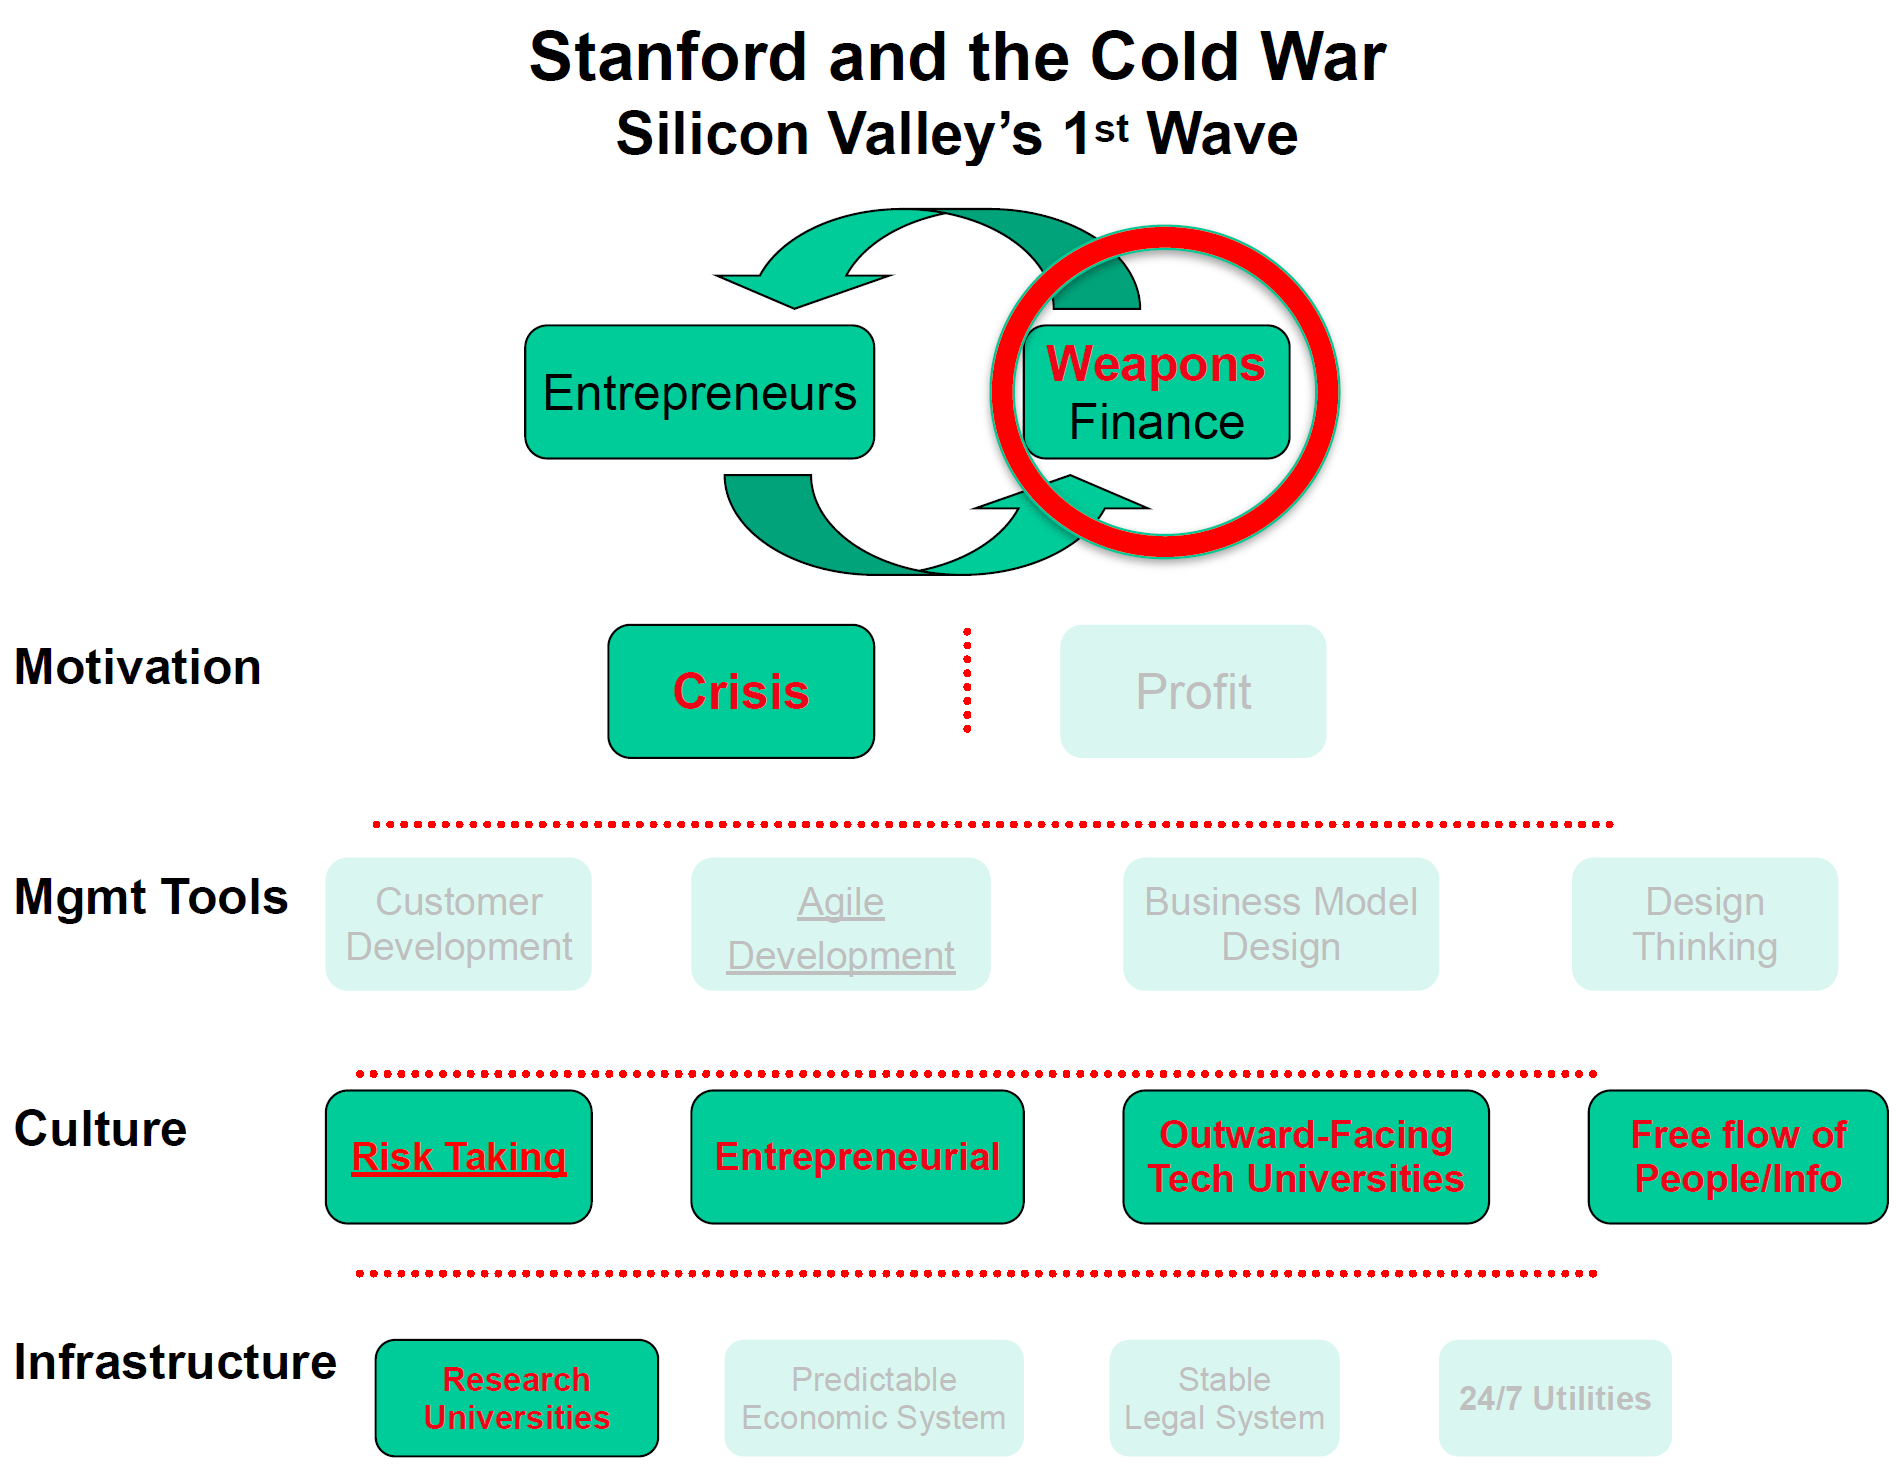
\includegraphics[width=0.7\textwidth]{Pictures/Stanford_cold_war_1.png}
\end{figure}

\begin{figure}[H]
    \centering
    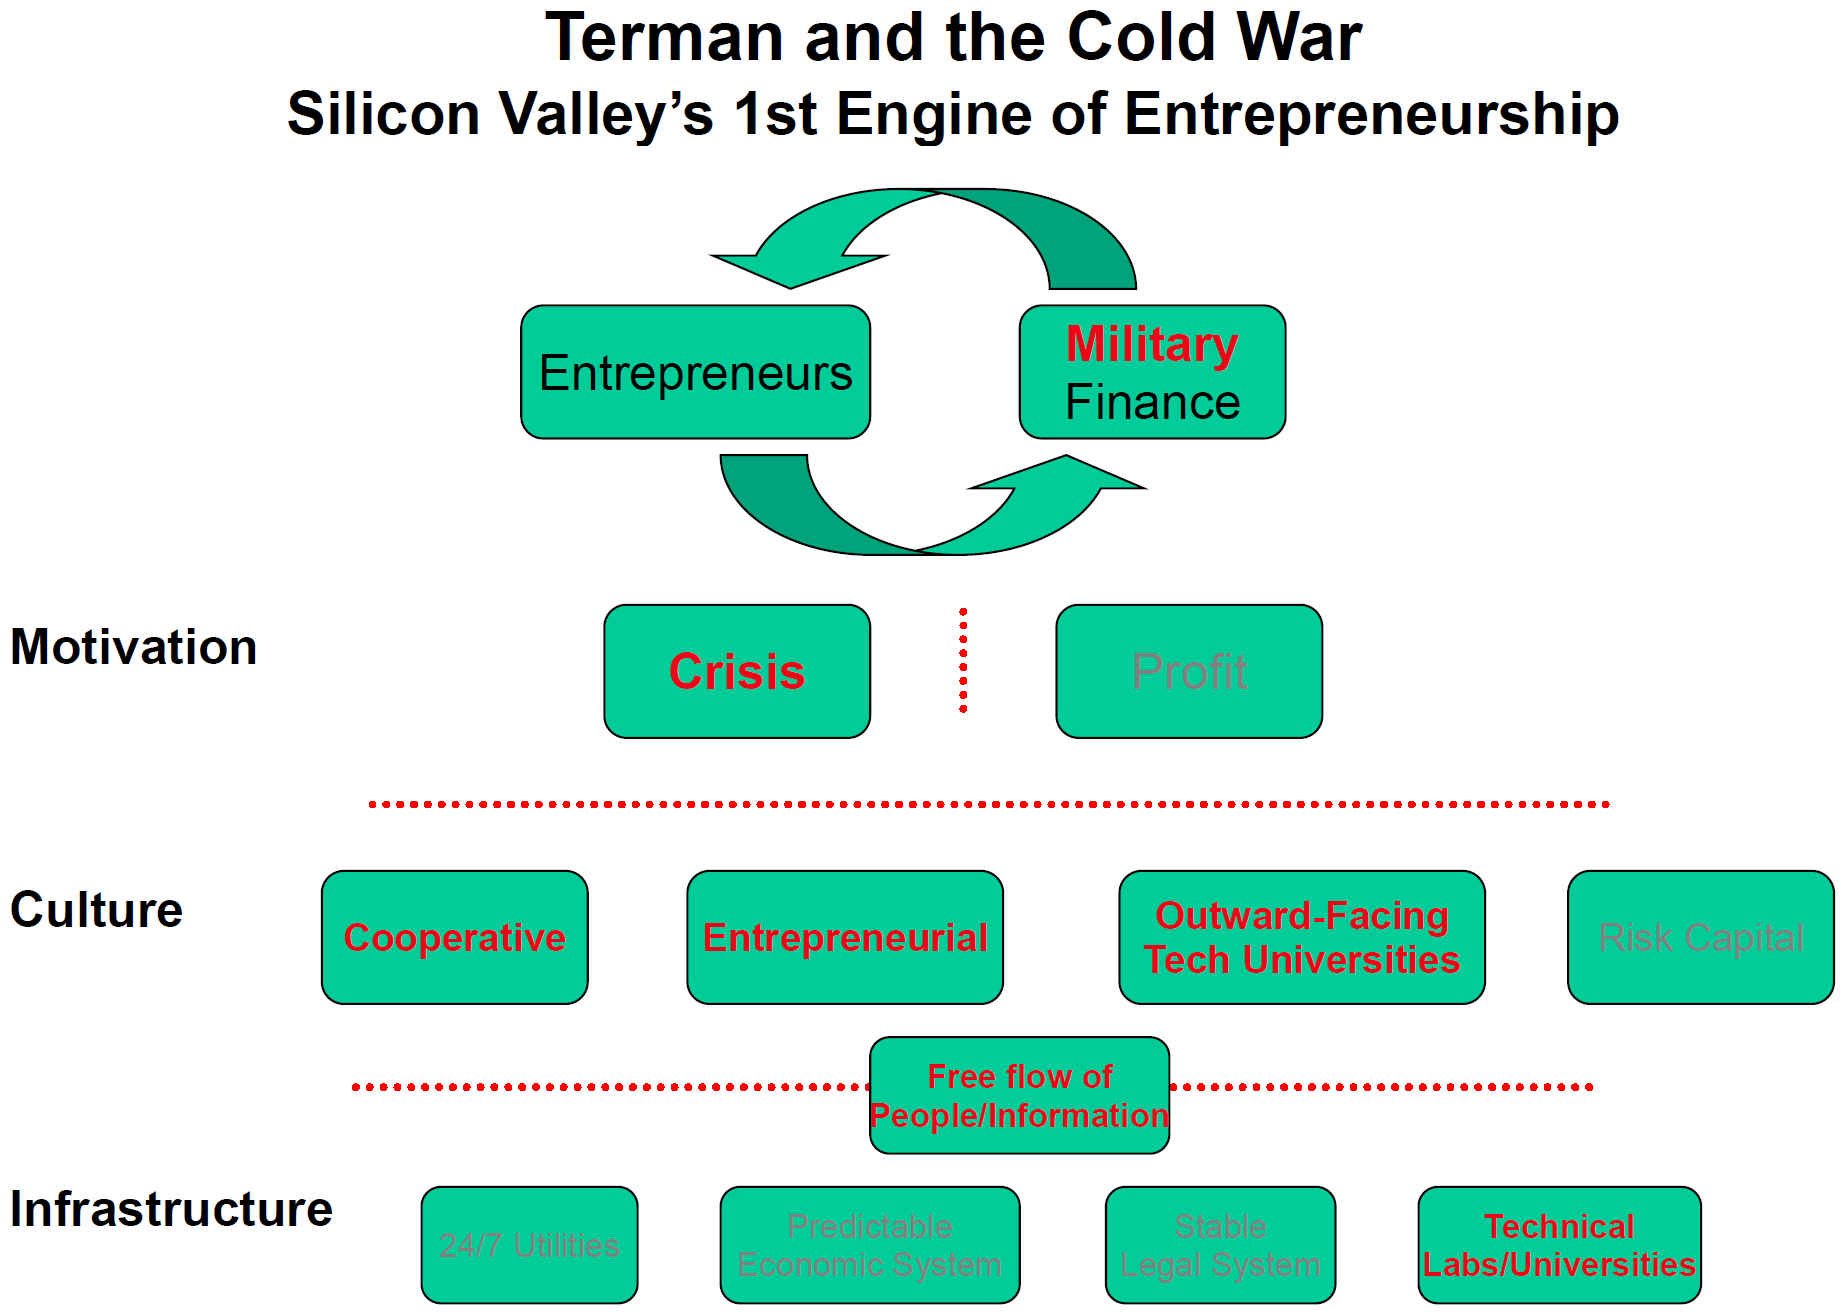
\includegraphics[width=0.7\textwidth]{Pictures/Stanford_cold_war_2.png}
\end{figure}


\paragraph{The End of Classified Work at Stanford}

\begin{itemize}
    \item In 1968, 35\% of Stanford research funding in electronics was for
        classified work
    \item 50\% of SRI's work was from DOD
    \item April 9, 1969 400 students occupy AEL
\end{itemize}

\paragraph{Shockley's Legacy}

\begin{itemize}
    \item Director of Navy anti-submarine warfare operations group at
        Columbia (1942-1943)
    \item Head of Radar Bombing training for Air Force (1943-1945)
    \item Deputy Director and Research Director of the Weapons System Evaluation
        Group in the Defense Department (1954-1955)
    \item Co-inventor of the transistor (Nobel Prize in 1956)
    \item Founded Shockley Transistor 1955
        \begin{itemize}
            \item First semiconductor company in California
        \end{itemize}
\end{itemize}

\subsubsection{The Rise of Venture Capital - The Limited Partnership}

\begin{itemize}
    \item Raise money from pension funds, private universities, wealthy
        individuals - the limited partners
    \item Investment professionals manage the fund - the general partners i.e.
        the VC's
        \begin{itemize}
            \item Compensate the general partners via the "2 and 20"
            \item 2\% management fee, 20\% carried interest (i.e. of the
                profits)
        \end{itemize}
\end{itemize}

\begin{figure}[H]
    \centering
    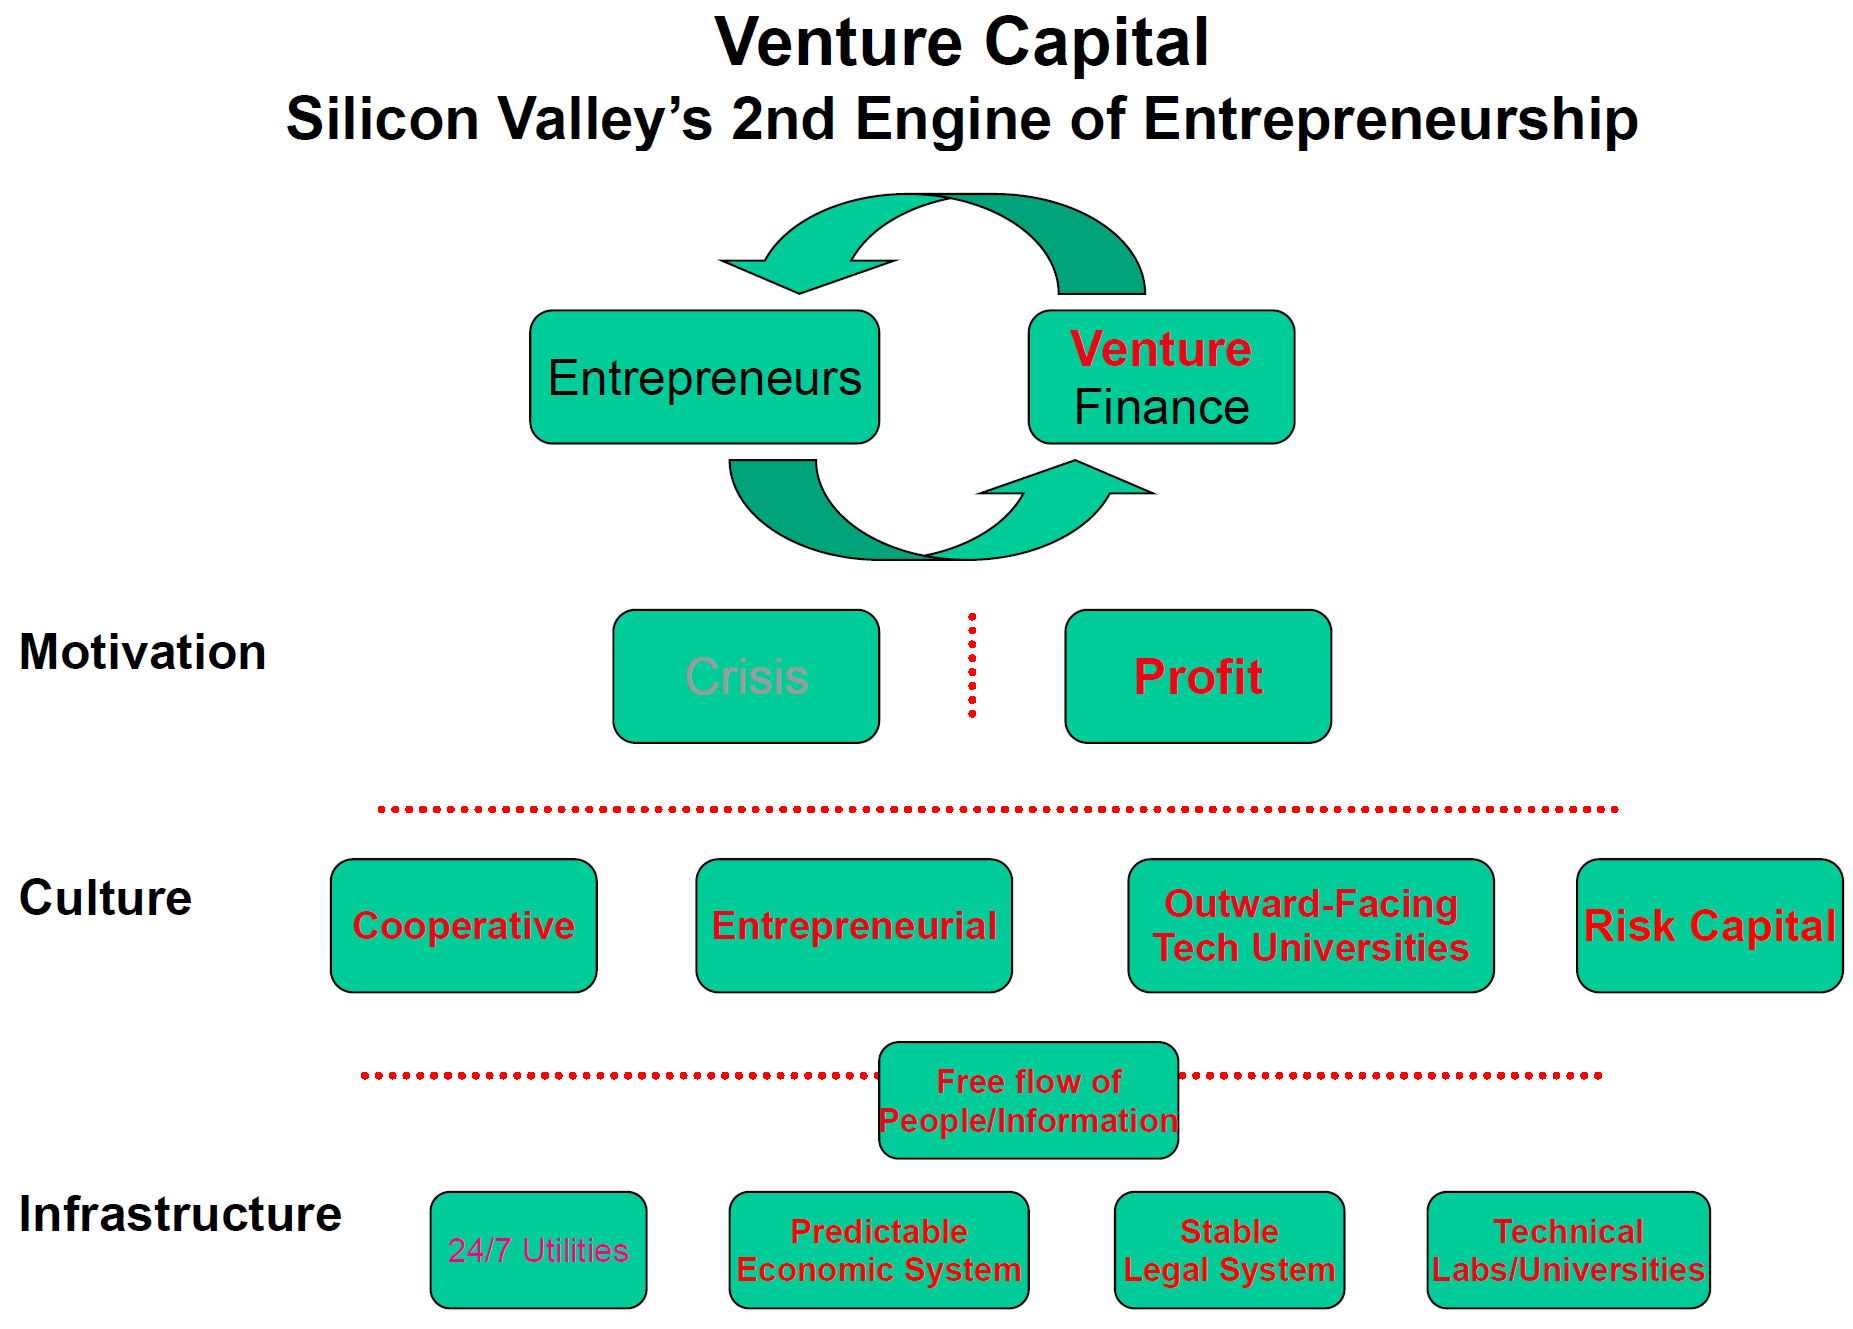
\includegraphics[width=0.8\textwidth]{Pictures/Venture_capital_silicon_valley.png}
\end{figure}

\subsubsection{Summary}

\begin{itemize}
    \item Terman/Stanford/Government responsible for entropreneurial culture
        of Silicon Valley.
    \item Military primed the pump as a customer for key Valley technologies
        \begin{itemize}
            \item Semiconductors, computers, Internet
            \item But very little technical cross pollination
        \end{itemize}
    \item Venture Capital turned the valley to volume corporate and consumer
        applications
\end{itemize}

Is there another "crisis" that will restart the valles's cycle of innovation?
Or will we continue to be profit driven?


\subsection{What is the State's role in the economy?}

\begin{enumerate}[a)]
    \item Set 'level' playing field then get out of the way
    \item solve 'market failures'
    \item something more interesting?
\end{enumerate}

The assumption: Private sector vs. public sector,
The new view: not only fixing the market but also shaping it.

Market failure policies don't explain the advent of key General Purpose
Technologies
\begin{itemize}
    \item 'mass production' system
    \item aviation technologies
    \item space technologies
    \item IT
    \item internet
    \item nuclear power
    \item nanotechnology
\end{itemize}

\begin{figure}[h]
    \centering
    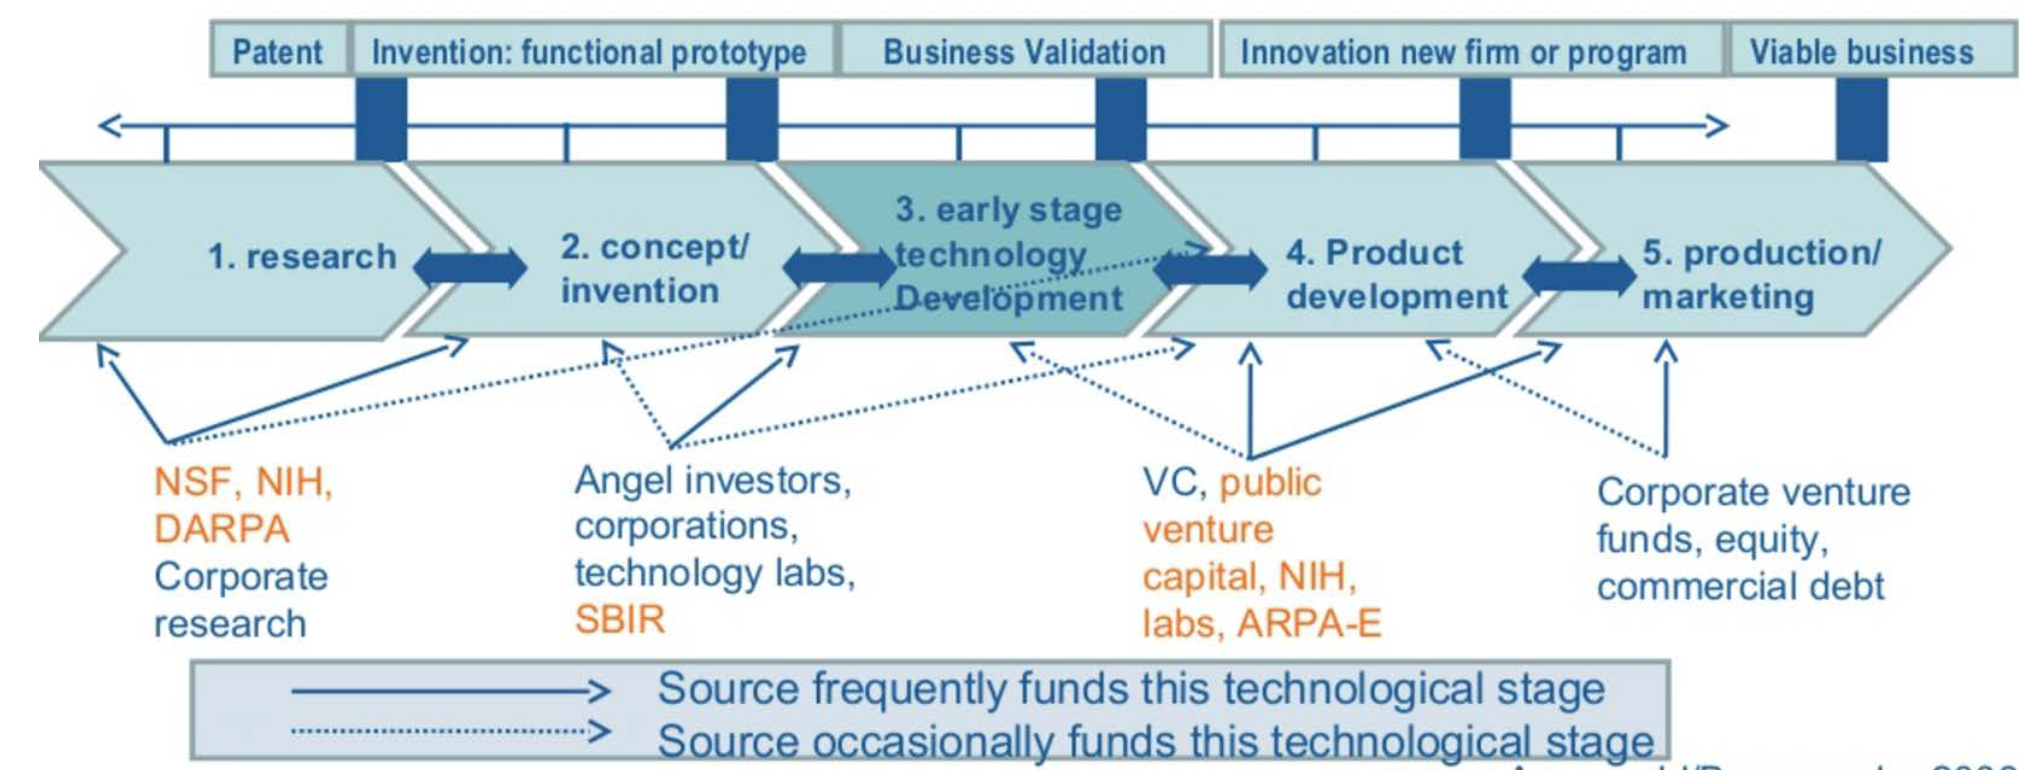
\includegraphics[width=0.7\textwidth]{Pictures/Mission_oriented_investment.png}
    \caption{Mission oriented investments along entire innovation chain}
\end{figure}

\subparagraph{Microships} powering the iPhone owe their emergense to the US
military and space programs, which made up almost the entire early market for
the breakthrough technology. In the 1960s, the government bought enough of the
initially costly chips to drive down their price 50x in a few short years,
enabling numerous new applications.

\subparagraph{Cellular communication} The early foundation of cellular
communication lies in radiotelephony capabilities advanced throughout the 20th
century with support form the US military.

\subparagraph{Internet} The technologies underpinning the Internet, which gives
the "smart phone" its smarts, were developed and funded by the Defense Department's
Advanced Research Projects Agency (DARPA) in the 1960s and 70s.

\subparagraph{GPS} was created/deployed in 1980s/90s by the military's
NAVSTAR satelite program and still today maintained via public funds.

\subparagraph{Multi-touch displays} that makes using an iPhone so intuitive has
the government's fingerprints all over it. The revolutionary interface was first
developed by a prilliant pair of universities of Delaware researchers supported
by NSF and CIA grants

\subparagraph{SIRI} was initially developed in DARPA.


\subsection{The Social Bubble Hypothesis}

"Enthusiastic supporters of an idea / a project / an opportunity weave a network
of reinforcing feedbacks based on exuberant anticipation that lead to widespread
endorsement and extraordinary commitment beyond what would be rationalized by a
standard cost-benefit analysis."

\vspace{1\baselineskip}

How to engineer useful bubbles for innovation!

\vspace{1\baselineskip}

The social Bubble Hypothesis: "innovation accelerator"

\begin{definition}
    A social bubble developing during a technological project is defined when
    several of the following symptoms are simultaneously present:
    \begin{enumerate}[(i)]
        \item strong growth of presence in the media, newspapers, books,
            blogs, gossips, cocktails\dots
        \item flow of venture capital and Wall Street investments
        \item accelerated price growth of corresponding firms trading on
            organized stock markets
        \item proliferation of venture of all kinds
    \end{enumerate}
\end{definition}

Three case studies so far: The US Apollo Program (1960-1969),
The Human Genome Project (1990-2003), The FuturICT Project (2010-2013)

\paragraph{The Human Genome Project}

\begin{itemize}
    \item In February 2001, Celera and HGP scientists published details of their
        drafts, describing the methods used and offering analysis of the
        sequence
    \item Improved drafts were announced and presented to the public in 2003,
        filling the open gaps
\end{itemize}

Anticipations of the commercial and medical applications of the HGP were highly
inflated. Today, it is acknowledged that insight into the genetic mapping and
sequencing effort is only seen as a starting point for future research in
biology and medicine. Contrary to claims during its development, the main fruits
of the Human Genome Project have been accruing to the research cummunity, and
almost nothing to medicine and the general public. But indirect technological
gains values at $>750$ Billions USD by Obama's administration.

\paragraph{Future social bubbles?}

\begin{itemize}
    \item biotech and nanotech, genomics, proteomics, personalised medicine
    \item Apps revolution (like pre-internet boom)
    \item open and big data revolution
    \item Green tech revolution
    \item Gas and oil Fracking
    \item Space frontier
    \item Ocean frontier
    \item Nuclear energy technology revolution
    \item Bitcoin
\end{itemize}

\paragraph{"Salvation and Profit": Deconstructing the Clean-Tech Bubble}

\begin{itemize}
    \item Form 2004 to 2008, a bubble formed in clean technologies, such as
        solar, biofuels, batteries, and other renewable energy sources.
    \item This clean-tech bubble can be rationalised through the lens of the
        Social Bubble Hypothesis, which holds that strong social interactions
        between enthusiastic supporters weave a network of reinforcing feedbacks
        that lead to widespread endorsement and extraordinary commitment by
        those involved.
    \item Detailed synthesis of the development of the clean-tech bubble, its
        history, and the role of venture capital and government funding in
        catalyzing it.
    \item Underlying narrative that was fueling the bubble.
    \item Evidence that the clean-tech bubble constituted an example of an
        innovation-accelerating process.
\end{itemize}

The clean-tech bubble was clearly a social bubble: the narrative of a "normal
imperative" to combat climate change and achieve "salvation", the ballooning
venture capital investments, and the massive government subsidies weaved a
network of self-reinforcing spirals that led to over-optimistic expectations,
excessive enthusiasm, and ovver-investments.

\vspace{1\baselineskip}

The question now arises whether the clean-tech bubble was - as it has been
historically the case for a number (but not all) bubbles - accelerated the
development, deployment, and diffusion of clean technologies. In other words,
did viable commercial and industrial infrastructure and products emerge after
the bust of the bubble?

\vspace{1\baselineskip}

Although the clean-tech bubble went burst, we can identify some factors that
indicate that the bubble did indeed catalyze technological progess in clean
and renewable energy technologies.

\vspace{1\baselineskip}

In essence, the clean-tech bubble of the mid-2000s catalyzed a massive decrease
in cost by excessively funding research and development in different clean-tech
sectors, such as solar or wind. While almost all of the clean-tech startups of
the last bubble failed, the clean-tech bubble, by decreasing prices and funding
innovation, massively de-resked clean and renewable energy technologies.
Solyndra, for example, failed because it was trying to merket a cutting-edge
new solar cell, which ended up being too expensive when the design costs started
to decrease. Today, solar or wind are no longer risky technologies and are now
even cost-competitive with legacy energy sources, such as gas or coal. This
decrease in costs and the elimination of technical risks of clean tech is now
catalyzing more investment opportunities, which, in turn, attracts new
entrepreneurs and investors, such as Softbank, Founders Fund, Sequoia Capital,
Y Combinator, and the two funds that were already investing in first clean-tech
boom-and-bust cycle, Kleiner Perkons and Khosla Ventures.


\subsection{Certain to Win}

\paragraph{John Boyd - USAF}
The fighter Pilot who changed the art of air warfare. Act fast and seem
unpredictable. "Forty-Second-Boyd": He was dubbed "Forty-second Boyd" for his
standing bet as an instructor pilor that, beginning from a position of
disadvantage, he could defeat any opposing pilot in air combat maneuvering
in less then forty seconds. He never lost.

\vspace{1\baselineskip}

Developed the Aerial Attack Study: After the study was declassified, foreign
pilots passing through Nellis took it home where it changed the way every air
force in the world flies and fights. Even today, more than 40 years later,
nothing substantial has been added to the Aerial Attack Study.

\vspace{1\baselineskip}

After a six-year assignment at Nellis, Boyd returned to collage for another
undergraduate degree. He went to the Georgia Institute of Technology where, one
night while studying for an exam in thermodynamics, he had the epiphany that
became his famous \textit{Energy-Maneuverability Theory}, or E-M Theory, as it
came to be known.

\vspace{1\baselineskip}

The E-M Theory changed everything that everyone thought they knew about fighter
combat. It enabled fighter pilots to evaluate their energy potential at any
altitude and at any maneuver. And, perhaps more importantly, the energy potential
of their adversary. It changed forever the way aircraft are fought in combat.

\vspace{1\baselineskip}

Boyd then used E-M as a design tool. Until E-M came along, fighter aircraft had
been designed to fly fast in a straight line or fly high to reach enemy bombers.
The F-X, which became the F-15, was the first Air Force fighter ever designed
with maneuvering specifications. Boyd was the father of the F-15, the F-16 and
the F-18.

\vspace{1\baselineskip}

America has dominated the skies for the past 30 years because of John Boyd.

\vspace{1\baselineskip}

After he retired, he developed a theory of combat that, according to Vice
President Dick Cheney who was Secretary of Defense at the time, was
responsible for America's swift and decisive victory in the Gulf war.

\begin{figure}[H]
    \centering
    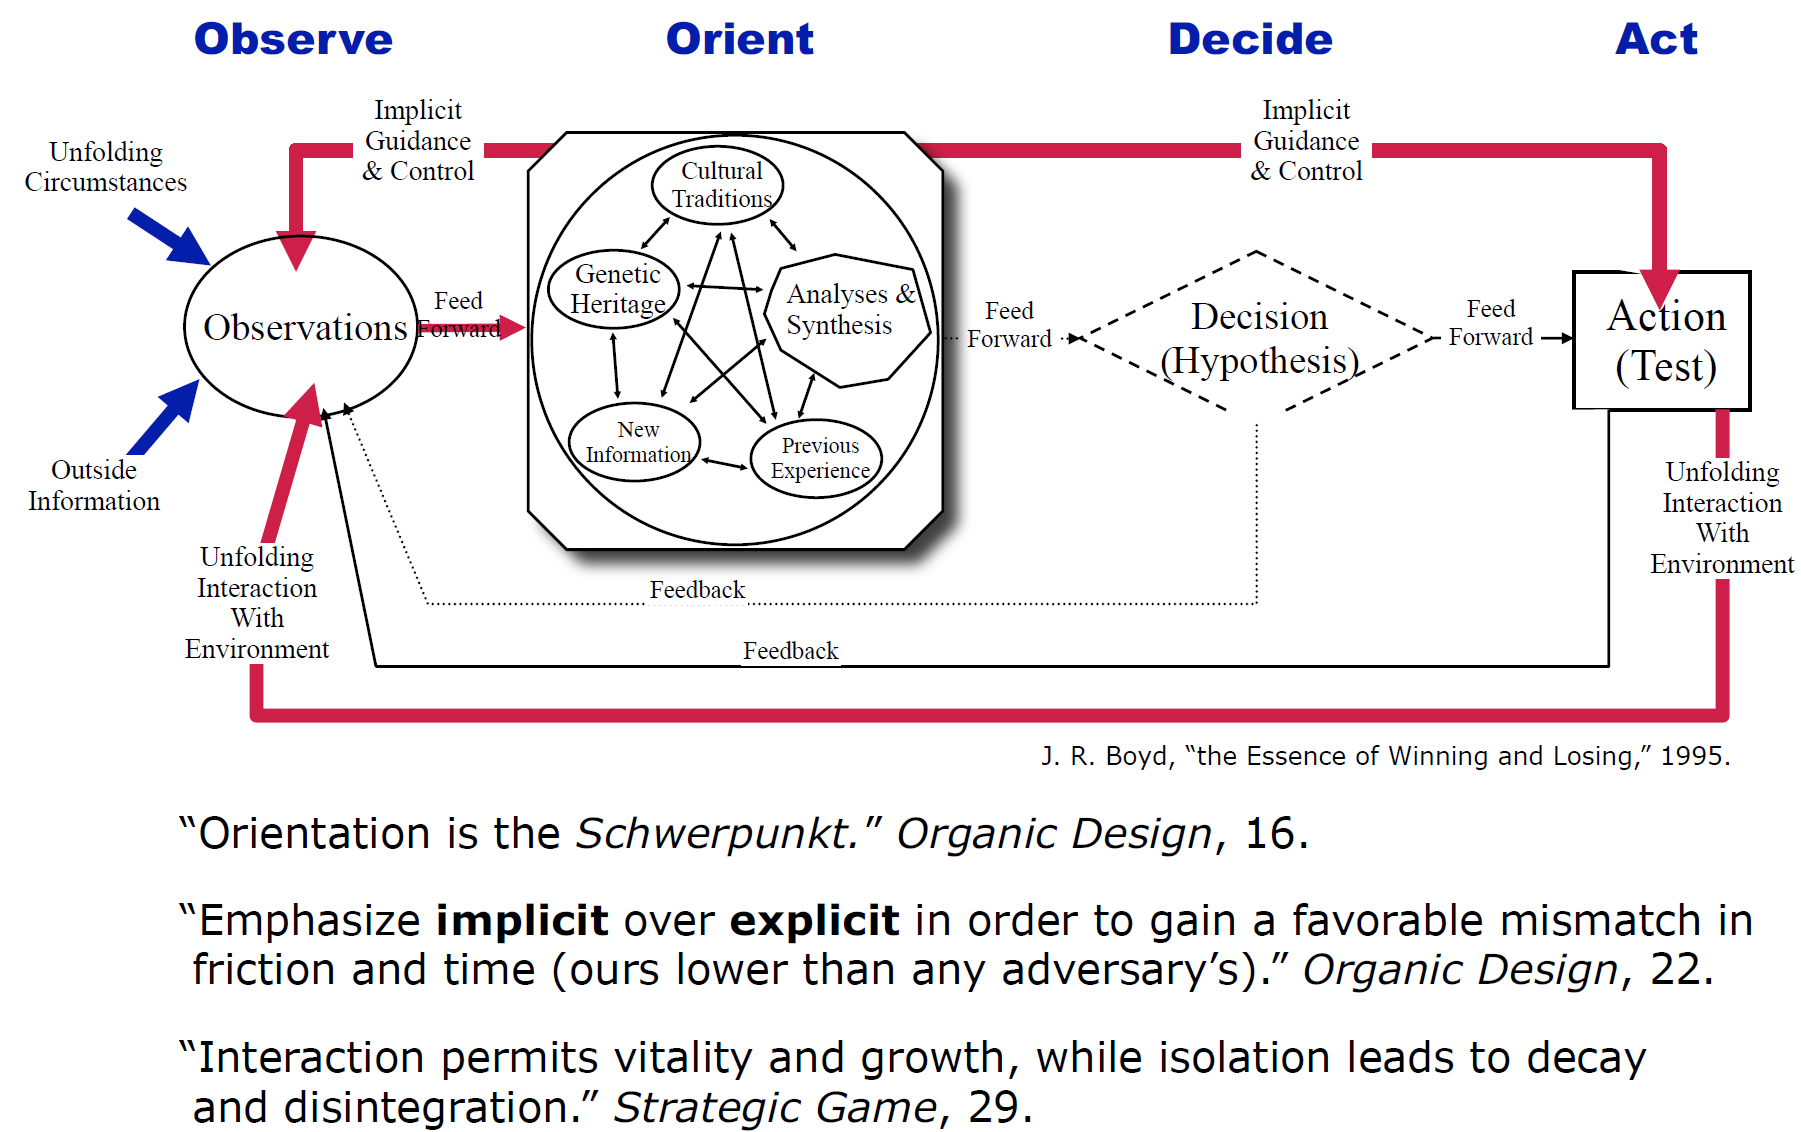
\includegraphics[width=0.8\textwidth]{Pictures/OODA.png}
\end{figure}

\begin{figure}[H]
    \centering
    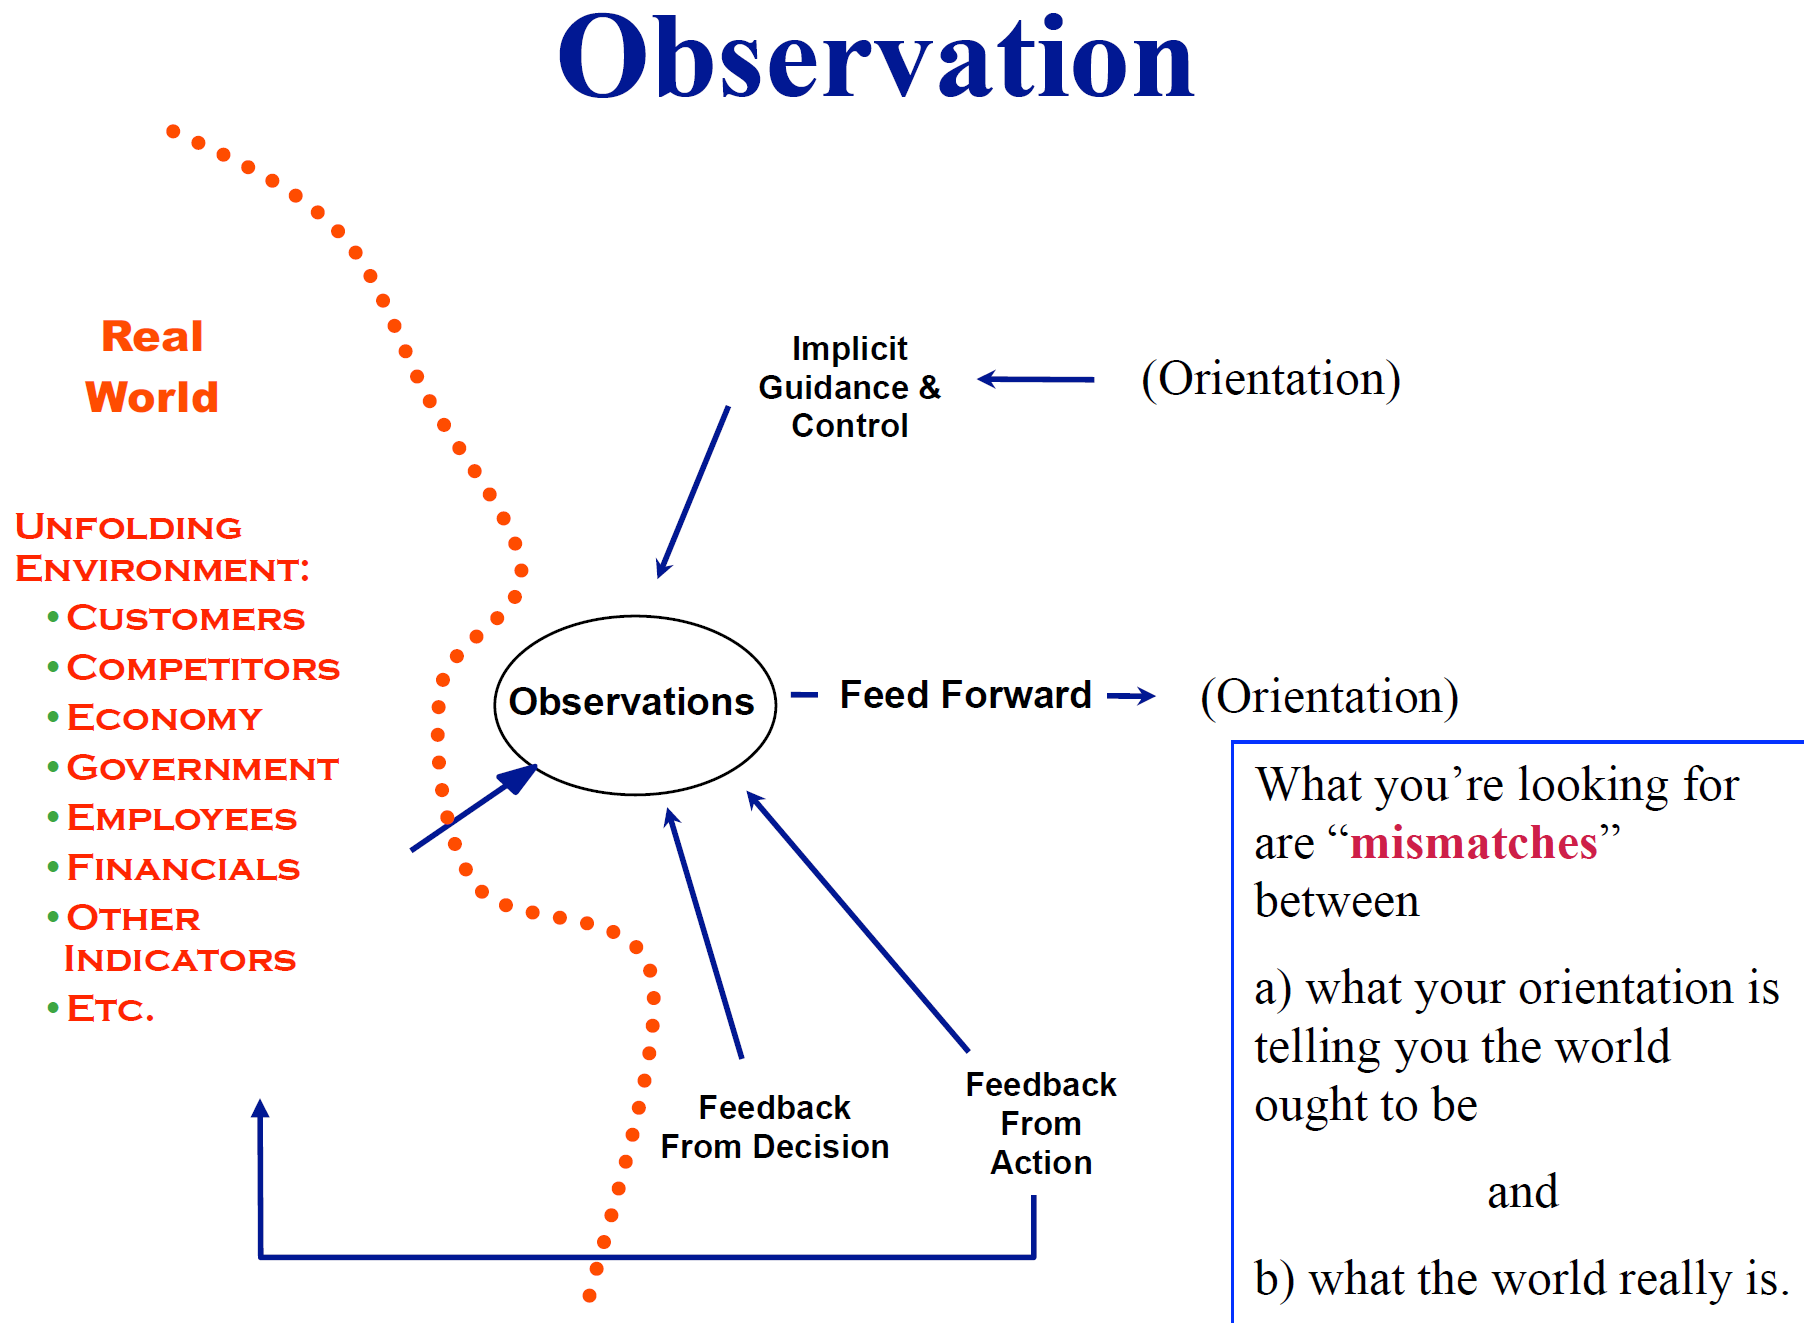
\includegraphics[width=0.7\textwidth]{Pictures/Observation.png}
\end{figure}

Wars don't always turn out as expected. Business doesn't eigher. But it's not
inevitable.

\paragraph{Time is special}

\begin{itemize}
    \item Time is the only physical parameter with a direction (the "arrow
        or time")
    \item You don't have an unlimited supply.
    \item Once it's gone, it's gone.
    \item Sure sign you're not using Boyd's strategies: you try to solve problems
        by throwing more time at them.
    \item I may lose a battle, I will never lose a minute - Napoleon
    \item A time-compressed company does the same thing as a pilot in an OODA
        loop\dots It's the competitors who act on information faster who is in
        the best position to win.
\end{itemize}

Using time as a weapon: The "H-Y War" (1981-1983)
\begin{itemize}
    \item Honda Motorcycles introduced or replaced 113 models, effectively
        turning over its entire product line twice.
    \item Yamaha, which also started about 60 models, was only able to manage
        37 changes in product line over the same 18 months.
    \item Observation: As a result, Honda was able to incorporate (and test
        in the marketplace) a much wider variety of styling \& technology. But
        that alone would not have been decisive.
\end{itemize}

Put it simple:
\begin{itemize}
    \item Good news is dangerous
    \item Bad news is the only thing that will save you, if:
        \begin{itemize}
            \item You find it before it finds you
            \item You correct your orientation
            \item You act upon it
        \end{itemize}
\end{itemize}

What determines OODA loop speed?
\begin{itemize}
    \item Ultimately, a moral climate/culture/environment that encourages
        people to use their initiatives to further the goals of the organization
    \item Under such a climate, people will solve the technical problems
\end{itemize}

Boyd's organizational climate: The principles of the Blitzkrieg
\begin{itemize}
    \item \underline{Fingerspitzengefühl} - Zen-like quality of intuitive
        understanding. Ability to sense when the time is ripe for action. Built
        through years of progressively more challenging experience.
    \item \underline{Einheit} - Has the connotation of "mutual trust" and
        implies a common outlook towards business problems. Built through common
        experience. Fingerspitzengefühl at the organizational level.
    \item \underline{Schwerpunkt} - Any concept that gives focus and direction
        to our efforts. In ambiguous situations, answers the question, "What do
        I do next?" Requires leadership.
    \item \underline{Auftragstaktik} - Tell team members what needs to be
        accomplished, get their agreement to accomplish it, then hold them
        strictly accountable for doing it - but don't prescribe how. Requires
        very high level of mutual trust.
\end{itemize}

Flowdown: Schwerpunkt for manufacturing:

The Toyota Production System, quite simply, is about shortening the time
it takes to convert customers orders into vehicle deliveries. This tells
everybody in Toyota manufacturing: "When in doubt, take the action that has
the biggest impact on order-to-delivery time".

\vspace{1\baselineskip}

Another Schwerpunkt:

Most CEOs are focused on achieving their financial and operational goals,
and on executing a strategy. But Apple's Steve Jobs believed his company's
ultimate advantage comes from its ability to make unique, or as he called
them, "insanely great" products. Jobs's entire company is focused on that
task.

\vspace{1\baselineskip}

Effective Forces play the Cheng / Ch'i Game
\begin{itemize}
    \item Sun Tzu: "Making armies able to take on opponents without being
        defeated is a matter of unorthodox (Ch'i) and orthodox (Cheng) methods\dots
        give rise to each other like a beginning-less circle - who could exhaust
        them?"
    \item Boyd: "\dots to gain a feel for the ways the cheng / ch'i game has
        been (and can be) played."
    \item Can be played on multiple levels, i.e., if opponent knows we like
        cheng / ch'i, we can exploit that fact also (Hitler at invasion of
        France, 1944)
\end{itemize}

